\documentclass[a4paper,draft]{article}

\usepackage[utf8]{inputenc}
\usepackage[T1]{fontenc}

\usepackage{lmodern}
\usepackage{amsmath}
\usepackage{amssymb}
\usepackage{stmaryrd}

\usepackage{mathtools}
\usepackage{amsthm}
\usepackage{thmtools}
\declaretheorem{theorem}
\declaretheorem{lemma}
\declaretheorem{corollary}
\declaretheorem[style=definition,qed=$\blacktriangle$]{example}
\declaretheorem[style=definition,qed=$\blacktriangle$]{definition}
\numberwithin{equation}{section}

\usepackage{enumitem}
\setlist[enumerate,1]{label=\alph*)}
\newlist{prfcases}{enumerate}{1}
\setlist[prfcases,1]{label={\it Case \arabic*.},align=left,leftmargin=\parindent,itemindent=*}

\newenvironment{isabelle}{\list{}{}\item\relax}{\endlist}
\newcommand{\iindent}{\-\hspace{1em}}

\usepackage{algorithm}
\usepackage[final]{listings}
\lstset{numbers=left,firstnumber=1,stepnumber=5,numberfirstline,
	basicstyle=\ttfamily\small,keywordstyle=\ttfamily\small\itshape,columns=flexible}

\usepackage{tikz}
\usetikzlibrary{shapes.geometric,matrix,decorations.pathreplacing}
\tikzset{itermtree/.style={level distance=6mm,sibling distance=10mm,%
	edge from parent/.style={draw,solid},every node/.style={solid}}}
\tikzset{pure/.style={draw,rectangle,inner sep=4pt,minimum size=5mm}}
\tikzset{term/.style={draw,circle,inner sep=1pt,minimum size=5mm}}
\tikzset{ap/.style={fill,diamond,inner sep=0pt,minimum size=6pt}}
\tikzset{subtrm/.style={draw,isosceles triangle,isosceles triangle apex angle=55,%
	shape border rotate=90,minimum height=10mm,anchor=north,child anchor=north}}
\tikzset{subtrmf/.style={subtrm,level distance=10mm,sibling distance=16.67mm}}
\tikzset{subtrmn/.style={subtrm,level distance=4mm,sibling distance=6.67mm}}
\tikzset{abbrv/.style={dashed}}

\usepackage[
	style=numeric,
	sorting=none,
	doi=false,
	urldate=long,
]{biblatex}
\addbibresource{bibliography.bib}

\usepackage[hidelinks]{hyperref}


\newcommand{\ldb}{\llbracket}
\newcommand{\rdb}{\rrbracket}
\newcommand{\todo}{\fbox{To do.}}

\newcommand{\oftype}{\mathrel{::}}
\newcommand{\funT}{\Rightarrow}
\newcommand{\abs}[2]{\lambda #1.\>#2}
\newcommand{\Imp}{\Longrightarrow}
\newcommand{\imp}{\longrightarrow}
\newcommand{\All}[2]{\bigwedge #1.\>#2}
\newcommand{\all}[2]{\forall #1.\>#2}
\newcommand{\tvar}[1]{{'\!\textit{#1}}}
\newcommand{\svar}[1]{\textit{?#1}}
\newcommand{\set}[2]{\{#1\mid #2\}}

\DeclareMathOperator{\pure}{\mathit{pure}}
\newcommand{\ap}{\diamond}
\DeclareMathOperator{\sterm}{\mathsf{term}}
\DeclareMathOperator{\spure}{\mathsf{pure}}
\DeclareMathOperator{\sivar}{\mathsf{var}}
\newcommand{\siabs}[2]{\mathsf{abs}\;#1.\>#2}
\newcommand{\sap}{\mathbin{\mathsf{`ap`}}}
\newcommand{\sapp}{\>}
\newcommand{\sabs}[2]{{\boldsymbol\lambda} #1.\>#2}
\newcommand{\tabs}[2]{{\boldsymbol\lambda}^\ast #1.\>#2}
\newcommand{\termeq}{=_{\alpha\beta\eta}}
\newcommand{\unlift}[1]{\left\downarrow #1\right.}
\DeclareMathOperator{\vars}{var}
\newcommand{\varseq}{\overrightarrow{\vars}}
\DeclareMathOperator{\abseq}{abs}


\hyphenation{Isa-belle}

\title{Applicative Functors in Isabelle/HOL: Notes}
\author{Joshua Schneider}

\begin{document}

\maketitle
\section{Introduction}\label{sec:introduction}

\subsection{Motivation}\label{subsec:motivation} % TODO change?

Interactive theorem provers emphasize the human aspect of mathematical work.
Rather than relying on fully automatic proof search, the user guides
the process with their own understanding~\cite{harrison07}.
This requires a sufficiently expressive interface with features beyond plain
logical calculus.
In particular, there exists a demand for automation and abstraction of
patterns~\cite{bourke12}.
It is thus common to extend proving environments with (sometimes
domain-specific) tools.

In this report we present a particular variant of lifting we have implemented
for the Isabelle/HOL proof assistant~\cite{npw02}.
The term ``lifting'' is used in different contexts, often informally.
It vaguely refers to the transfer of mathematical objects between domains,
while preserving a certain relationship.
A concrete example are lifts of paths in topology. % TODO cite
There is also an existing Isabelle package~\cite{huffman13}, which lifts
definitions to quotient types.
Here we consider a slightly different meaning of lifting:
The transfer of operations and their properties to generic structures.
Since HOL is a typed logic, it is natural to represent these structures as
parametric types.
Let us look at a simple example.

\begin{example}\label{exmp:set-intro}
For each type $\alpha$ there is a corresponding type $\alpha\,\mathit{set}$
of sets with elements from $\alpha$.
Addition $(+)$ is a binary operator defined on natural numbers, amongst others.
How could addition of sets of natural numbers be defined, such that some
relation to $+$ remains?
The canonical way to combine two sets into a set of pairs is the cartesian
product.
Therefore, we define
\begin{equation}\label{eq:set-plus-exp}
	X \oplus Y = \set{x + y}{x \in X,\, y \in Y}.
\end{equation}
We interpret $\oplus$ as the lifting of $+$ to sets.
Note that similar definitions are possible for other operators like
multiplication, and also other element types such as real numbers.
A property of addition is associativity,
\begin{equation}\label{eq:plus-assoc}
	\all{x y z}{(x + y) + z = x + (y + z)}.
\end{equation}
It can be translated to sets of natural numbers,
\begin{equation}\label{eq:set-plus-assoc}
	\all{X Y Z}{(X \oplus Y) \oplus Z = X \oplus (Y \oplus Z)},
\end{equation}
where it holds as well, as one can check with a slightly laborious proof.
The two sides of the latter equation can be regarded as functions with three
arguments.
They are the lifted counterparts of the former equation.
\end{example}

Hinze~\cite{hinze10} came across similar patterns and proceeded to investigate
the conditions under which lifted equations are preserved.
He noticed that lifting can be defined in an intuitive fashion if the target
structure is an applicative functor~\cite{mcbride08}.
These come with two constants, usually denoted $\pure$ and $\ap$ (``ap''),
which lift a single object and the notion of function application, respectively.
Applicative functors must also satisfy some properties, which we restate in
Section~\ref{subsec:applicative}.

\addtocounter{example}{-1}
\begin{example}[continued]
Back to sets, we obtain an applicative functor if $\pure$ is the singleton set
constructor $x \mapsto \{x\}$;
$F \ap X$ takes a set of functions $F$ and a set of arguments $X$
with compatible type, applying each function to each argument:
\[ F \ap X = \set{f x}{f \in F,\, x \in X}. \]
Now we can express lifted addition directly in terms of the base operation:%
\footnote{As customary in HOL, we treat binary operators as curried functions.}
\[ X \oplus Y = \pure{(+)} \ap X \ap Y. \]
(The operator $\ap$ is left-associative.)
This definition is equivalent to the previous one \eqref{eq:set-plus-exp},
but not specific to sets anymore.
\end{example}

As we have seen earlier, lifting can be generalized to equations.
One of Hinze's results is that a fundamental relationship exists between the
associative properties \eqref{eq:plus-assoc} and~\eqref{eq:set-plus-assoc}%
---the lifted form can be proven for all applicative functors, not just
$\mathit{set}$.
Moreover, this is possible for other equations as well, but not all equations
can be lifted in all idioms, though.
Stronger conditions are required if the list of quantified variables is
different for each side of the equation.
(The left-to-right order is relevant, but not the nesting within the terms.)
These conditions must basically ensure that the functor does not add ``too many
effects'' which go beyond the simple embedding of a base type.
Such effects may be evoked if a variable takes an impure value, i.e., a value
which is not equal to $\pure x$ for any $x$.
Hinze showed that sufficient conditions can be expressed in terms of combinators
as known from combinatory logic.

\begin{example}\label{exmp:set-counterexmp}
We try to lift the fact that zero is a left absorbing element for
multiplication of integers, $\all{x \oftype \mathit{int}}{0 \cdot x = 0}$,
to sets.
Note that the variable $x$ occurs only on the left.
But the lifted equation does not hold: If $x$, now generalized to
$\mathit{int}\,\mathit{set}$, is instantiated with the empty set, then
\[ \pure{(\cdot)} \ap \pure 0 \ap \{\} = \{\} \ne \pure 0. \]
Here the effect of $\{\}$ is that it cancels out everything else if it occurs
somewhere in an idiomatic expression.
This makes it impossible to lift any equation with a variable occuring only on
one side to $\mathit{set}$.
We will see that other functors permit this lifting.
\end{example}

Our primary goal is to provide an Isabelle/HOL proof method which reduces
lifted equations to their base form.
The method can be instantiated for arbitrary applicative functors.
Then the user is able to prove the lifted equations directly without having to
invent a specific proof strategy, or even simulate the approach taken here.
We have further extended the idea of combinators as building blocks for lifting.
The package supports several combinator sets which functors may exhibit,
each capable of lifting different sets of equations.

Apart from the theoretical appeal of the method, the resulting proof text is
usually more concise, due to the higher level of abstraction.
Applicative functors are in fact quite common, thus we hope that our tool
can be reused elsewhere.
A particular motivation are arithmetic operations on streams (infinite lists)
and infinite trees.
We have proven some of their properties as an example of our package.
\todo


\subsection{Proving with Isabelle/HOL}\label{subsec:isabelle}

Isabelle was originally designed as a framework for interactive theorem
proving, without being restricted to a specific logical system~\cite{paulson90}.
However, one chooses a particular object-logic in order to construct a theory
and prove theorems.
In this paper, we focus on the Isabelle/HOL object-logic~\cite{npw02}.
It implements the higher-order logic which was used in the HOL~system,
another proving environment~\cite{gordon93}.
Isabelle/HOL (or HOL from here~on) is arguably the most popular object-logic
of Isabelle, as it comes with an extensive library of readily formalized
mathematics.
It also supports modelling of functional programs by means of datatypes and
recursive functions, making it suitable for verification tasks. % TODO cite?

The basis of HOL is a slightly extended variant of simply-typed lambda calculus.
Therefore, every object (and every term representing such an object) has a
certain type attached to it.
We use lower-case greek letters $\alpha$, $\beta$, $\gamma$ as meta-variables
for types.
The language of types consists of base types, type variables, and compound
types.
Base types are represented by their name and include fundamental types like
the booleans $\mathit{bool}$ and the natural numbers $\mathit{nat}$.
Type variables stand for an arbitrary types.
In Isabelle syntax, they are distinguished by a prefixed `$'$', e.g.
$\tvar{a}$, $\tvar{b}$, $\tvar{c}$.
The polymorphism in HOL is quite restricted, though, because higher-ranked
types cannot be expressed:
There is no explicit quantifier on the type level.
This rules out functions which take a polymorphic function as an argument and
apply it to values of different types.
Compound types are built up of a type constructor and a list of types.
The type constructor determines the number of argument types.
For example, the unary type constructor $\mathit{set}$ denotes sets with
elements of a certain type.
The argument is written on the left as in $\mathit{nat\,set}$, the type of
sets of natural numbers.
Multiple types are written in parentheses: $(\alpha, \beta) \mathit{fun}$.
$\mathit{fun}$ is the special type constructor for (total) functions from
$\alpha$ to $\beta$.
More commonly, the infix operator $\funT$ is used.
It is right-associative, i.e. $\alpha \funT \beta \funT \gamma$ is notation for
$(\alpha, (\beta, \gamma) \mathit{fun}) \mathit{fun}$.
Note that type constructors are different from types and must always be
concrete.
In particular, it is not possible to use a variable in place of a type
constructor!

Terms follow the standard rules of lambda calculus.
Atomic terms are constants and variables.
Application of a function $f$ to an argument $x$ is written $f\,x$.
Functions with multiple arguments are commonly curried in HOL;
we can drop parentheses accordingly: $f\,x\,y$ is the same as $(f\,x)\,y$.
Abstraction of a term $t$ over the variable $x$ is written $\abs{x}{t}$.
Terms must be well-typed, of course.
The types of variables and polymorphic constants can usually be omitted, since
they are inferred automatically.
Explicit type constraints are denoted by $t \oftype \alpha$ and may occur
anywhere in a term.
While all terms are represented internally roughly as shown above, Isabelle
comes with extensible notation support.

\begin{example}\label{exmp:hol-terms}
We already introduced the type $\mathit{nat}$.
Number literals can be used directly.
Common arithmetic operators are available, like%
\footnote{These functions actually have a more generic type (they are
overloaded). We will look at this later on.}
$\mathit{plus} \oftype \mathit{nat} \funT \mathit{nat} \funT \mathit{nat}$.
We can also use infix operators:
\[ \abs{(x \oftype \mathit{nat})\,y}{1 + x * y} \]
is a function which multiplies two natural numbers and adds one to the result.
Another important type family are sets.
They can be specified as finite collections $\{\}$, $\{a, b, c\}$ etc., and
by using set comprehension:
Let $P$ be a predicate $\alpha \funT \mathit{bool}$.
Then $\{x.\; P x\}$ is the set of those values $x \oftype \alpha$ such that
$P x$ is true, and $\set{f x}{x.\; P x}$ is the image of that set under $f$.

Logical formulas are centered around truth values.
Thus, the usual connectives like conjunction $\land$ and implication $\imp$
operate on type $\mathit{bool}$.
Quantifiers work just as expected: The term
\[ \all{(x \oftype \mathit{nat})\,y}{x + y = y + x} \]
states that addition of natural numbers is commutative.
Note that $=$ is just another operator of polymorphic type
$\tvar{a} \funT \tvar{a} \funT \mathit{bool}$.
Internally, quantifiers are represented as constants applied to lambda
abstractions, which handle the variable binding.
\end{example}

In order to achieve the goal of supporting different object-logics,
Isabelle contains an immediate layer, the meta-logic Pure.
It is an ``intuitionistic fragment of higher-order logic''~\cite[27]{isar-ref}.
In Pure itself there is only the type $\mathit{prop}$ of propositions.
A term of this type combined with a proof relative to some context forms a
\emph{theorem}.
For now, the context is an abstract entity which may contain local hypotheses.
Assumptions can also be recorded explicitly in a proposition, using
meta-implication $\Imp$.
Note that this is technically different from HOL's implication $\imp$,
though there are theorems which allow conversion between the two.
The meta-quantifier $\bigwedge$ denotes universal quantification (with a
similar relationship to $\forall$); it is used to restrict the scope of
variables in assumptions.
Meta-equality $\equiv$ is the third main operator of Pure.
The generic rewriting and simplification tools work with such equations.
Again, conversion with $=$ is possible.
Object-logics embed their own notion of a proposition into Pure via
a truth judgement.
In HOL, this is the constant $\mathit{Trueprop} \oftype \mathit{bool \funT prop}$,
which turns an object-level formula into a proposition stating that said
formula is indeed true.
It is usually left implicit.
See \cite[Chapter~2]{implementation-ref} for further details about Pure.

Pure has two main uses within the Isabelle framework: representation and
manipulation of deduction rules, and goal states.
For the former, consider the traditional introduction rule for conjunction,
\[ \frac{\Gamma_1 \vdash P \qquad \Gamma_2 \vdash Q}{\Gamma_1 \cup \Gamma_2 \vdash P \land Q}, \]
which we want to turn into a theorem.
Deduction in Isabelle handles the contexts $\Gamma_i$ automatically, and
therefore do not have to be stated in the corresponding proposition.
The dependency of the conclusion $P \land Q$ on the hypotheses $P$ and $Q$
translates to repeated meta-implication.
This gives us the proposition
\[ \All{P Q}{P \Imp Q \Imp P \land Q} \]
(the $\mathit{Trueprop}$ markers have been omitted, and $P$, $Q$ range over
$\mathit{bool}$).
There is one quirk, however.
The outermost meta-quantified variables (and all type variables) % FIXME
are turned into schematic variables, which are free variables distinguished by

the prefix $\svar{}$.
Thus, the introduction rule as it is supplied by HOL appears as
\[ \mathtt{conjI}:\quad \svar{P} \Imp \svar{Q} \Imp \svar{P} \land \svar{Q}. \]
Schematic (type) variables are eligible for instantiation during
\emph{resolution}, which is Isabelle's primary tool for proof construction.
Resolution combines two rules (theorems), identifying an assumption of the
second with the conclusion of the first by higher-order unification.
Additionally, the first rule is brought into the context of that assumption.

A goal state is a theorem that represents a partially completed proof of some
proposition, the goal.
While the proof is incomplete, the remaining subgoals are tracked as
assumptions.
Proof steps transform the goal state.
The proof is finished once only the goal remains.

% TODO ML

In contemporary use of Isabelle, user input to the system is expressed in
the Isar language~\cite{wenzel99,wenzel02,isar-ref}.
It aims to encode proofs in a way that is formal, i.e. has precise semantics,
but still resembles informal patterns of reasoning.
The basic organization unit in Isar is a \emph{theory}.
The body of a theory consists of a sequence of commands, which consecutively
augment the logical context by declarations of various kinds.
Other theories may be imported in the beginning, leading to a acyclic graph
of theory dependencies.
Commands constitute the so-called outer syntax of Isar.
Terms and types occuring within them are parsed separately, according to the
inner syntax.
They are usually embedded in quotes `\texttt{"}\dots\texttt{"}' to disambiguate
them.
In certain cases, a command may put the theory state into proof mode.
% TODO goal, subgoal, nesting
After a proof is finished, the associated goal becomes a \emph{fact}.
% TODO facts by assumption

Some commonly used specifications are:
\begin{itemize}
\item The \textbf{definition} command introduces new constants by means of
	defining equations.
\item \todo{} \textbf{datatype}, \textbf{primrec}
\item Facts can be given names for further use in proofs.
	The canonical command for this is \textbf{lemma} and its variants
	\textbf{theorem} and \textbf{corollary}.
\item \todo{} \textbf{locale}?
\end{itemize}

Finally, there two syntactical categories which are repeatedly used in commands:
\emph{Proof methods} denote (possibly parameterized) operations on the goal state.
\emph{Attributes} invoke further processing steps on facts, either transforming
them or causing additional declarations.

% TODO
% - Isar example

% TODO
% LCF => extensibility?


\subsection{Applicative Functors and Lifting}\label{subsec:applicative}

Applicative functors were introduced by McBride and Paterson~\cite{mcbride08}
in order to abstract a recurring theme they observed in the programming language
Haskell.
In fact, their findings already included some examples of lifting.
They defined an applicative functor as a unary type constructor $f$ with
associated constants
\begin{align*}
	\pure_f &\oftype \alpha \funT \alpha f, \\
	(\ap_f) &\oftype (\alpha \funT \beta) f \funT \alpha f \funT \beta f.
\end{align*}
We omit the subscripts if the functor is clear from the context.
Moreover, the following laws must be satisfied:
\begin{align*}
	\tag{identity} \pure{\mathit{id}} \ap u &= u \\
	\tag{composition} \pure{(\cdot)} \ap u \ap v \ap w &= u \ap (v \ap w) \\
	\tag{homomorphism} \pure{f} \ap \pure x &= \pure{(f x)} \\
	\tag{interchange} u \ap \pure{x} &= \pure{(\abs{f}{f x})} \ap u
\end{align*}
We have already seen how the two constants can be used to build terms.
McBride and Paterson coined the term ``idiom'' to refer to a particular
interpretation of such terms.
In line with Hinze, we will use ``applicative functor'' and ``idiom''
interchangeably.

The identity type constructor defined by $\alpha\,\mathit{id} = \alpha$ is a
trivial applicative functor for $\pure{x} = x$, $f \ap x = f x$.
We can take any abstraction-free term $t$ and replace each constant $c$ by
$\pure{c}$, and each instance of function application $f x$ by $f \ap x$.
The rewritten term is equivalent to $t$ when interpreted in the identity idiom.
By choosing a different idiom, we obtain a different interpretation of the same
term structure.
In fact, this is exactly how we define the lifting of $t$.
However, the terms we are interested in can also contain variables:
Equations such as~\eqref{eq:plus-assoc} are universally quantified.
For the purpose of lifting, we ignore quantifiers and treat their variables
as free.
Like in Example~\ref{exmp:set-intro}, the variables of lifted equation should
range over the lifted type.
Note that these can take impure values.
A term consisting only of $\pure$ and $\ap$ applications and free variables is
then called an \emph{idiomatic expression}.

Every idiom is a functor, of course, and thus can be mapped over.
One obtains an equivalent formalization of idioms:
\begin{alignat*}{2}
	\mathit{map}_f &\oftype (\alpha \funT \beta) \funT \alpha f \funT \beta f, &\qquad
		\operatorname{\mathit{map}}_f\,g\,x &= \pure g \ap x, \\
	\mathit{unit}_f &\oftype () f, &\qquad \mathit{unit}_f &= \pure{()}, \\
	(\star_f) &\oftype \alpha f \funT \beta f \funT (\alpha, \beta) f, &\qquad
		x \star_f y &= \pure{(\abs{x y}{(x,y)})} \ap x \ap y.
\end{alignat*}
Some of Hinze's proofs make use of these definitions.
Dealing with product types can be a bit cumbersome in HOL, though.
The curried interface therefore seems to be a better choice, and we will
focus solely on that.

Every monad is an applicative functor.
Monads are a common mechanism for handling effects in functional
programming~\cite{wadler95}.
Such being the case, they are also useful for modelling in the context of
verification.
The difference between monads and applicative functors is that the latter
do not allow sub-computations to depend on previous results.
From there we get quite a few example idioms:
Sum types with one variable type (known as \textsf{Either} in Haskell),
the reader monad or environment functor, the state monad, and parser combinators.
Hinze originally worked on streams and infinite trees~\cite{hinze08,hinze09},
which we already mentioned.
We conclude that there are indeed relevant instances of idioms to which we
can apply our proof method.


\subsection{Contributions and Overview}\label{subsec:contrib-overview}

\todo

\chapter{Requirements and Basic Design}\label{sec:design}

\section{Requirements}\label{subsec:requirements}

Our primary goal is to implement an Isabelle/HOL proof method which reduces
lifted equations to their base form.
This proof method should be generic and work with arbitrary idioms.
The following is the minimal set of user actions we shall support:

\begin{enumerate}
\item Declare applicative functors to the theory context.
	Given a type constructor $f$, the functions $\pure_f$ and $\ap_f$, and
	proofs for the relevant functor laws, the functor is registered with the
	package such that it can be used in subsequent invocations of the
	proof method.
\item Prove lifted equations $a'[\vec{x}] = b'[\vec{x}]$, where $a'$ and $b'$
	are idiomatic expressions with free variables $\vec{x}$, using the base
	equation $\all{\vec{y}}{a[\vec{y}] = b[\vec{y}]}$.
	More precisely, if there is a subgoal stating the former, applying the
	proof methods transforms the goal state to the latter.
	The functor should be either detected automatically, or specified by
	the user.
\end{enumerate}

The first requirement ensures that our package is reusable, while the second
is the core functionality.
However, usability is also a concern: In the realm of interactive theorem
proving, it is not sufficient to just verify formal objects---we are not
extending the logic, after all, but providing a shortcut for a certain
principle.
We must balance the clarity of the resulting proof document and the amount of
work that the user has to put into developing a proof.
The following features are possible extensions which may help in this regard:

\begin{enumerate}
\setcounter{enumi}{2}
\item\label{itm:feat-const}
	Declare lifted constants and other terms to the theory context.
	Generally speaking, if a term $t$ with free variables $v_i$ can be expressed
	as $\pure t' \ap v_1 \ap \cdots \ap v_n$ for some $t'$, then the
	corresponding equation can be registered.
	The lifting proof methods rewrites with these equations at the beginning,
	such that the base equation will refer to $t'$.
	This way, the user does not have to transform everything into idiomatic
	format first.
\item\label{itm:feat-flex}
	More flexibility regarding the logical structure of the input proposition.
	This includes bound variables (quantified by $\forall$ or $\bigwedge$),
	complex subgoals with premises, and cases where the conceptual variables
	of the lifted equation have been subsituted by some terms.
\item\label{itm:feat-tools}
	Related proof methods and attributes, for example for forward lifting
	of proven base equations.
\item\label{itm:feat-debug}
	Inspection and tracing output.
	This is particular useful if something does not work as expected.
\item\label{itm:feat-xprops}
	Extend the notion of lifting beyond equations.
	It is possible to define lifting for other logical operators.
	For example, the cancellation law $a + b = a + c \longrightarrow b = c$
	consists of two equations, joined by implication.
	We can interpret it in different domains, e.g., for integers and for
	streams of integers with element-wise addition.
	In this example, the law is true for both interpretations.
	We are not able to handle such propositions with just a method for
	equations, though.
	% TODO example may fit better somewhere else?
\end{enumerate}

The current version at the time writing supports \ref{itm:feat-const} and
\ref{itm:feat-flex}, as well as \ref{itm:feat-tools} and \ref{itm:feat-debug}
to some extent.
In the remainder of this section, we will explain the design decisions we
have made in order to fulfill the requirements.
Furthermore, the registration infrastructure and the basic proof approach are
explained.


\section{Choice of Embedding}\label{subsec:embedding}

The basic way of proof composition in Isabelle is resolution with a proven
theorem, using it as a rule of inference.
Here we argue that it is not possible to prove lifting as a single theorem, and
then we discuss potential remedies.
We are interested in applicative functors on the type level, where application
is based on the standard function space.
Therefore, each idiom comes with a type family which is indexed by a
distinguished type variable, and the related functions and laws are polymorphic
in this index.
This is the natural form of idioms in the HOL libraries; all examples
in~\ref{subsec:applicative} are parametric datatypes.
The proof method should work directly with equations of these idioms.
Regardless of the mechanism of proof construction, it needs a type constructor
as a parameter.
This concept is foreign to the type system of Pure and HOL---%
we already referred to the fact that type constructors are fixed.
Another issue is the lack of polymorphism in the inner logic:
We cannot have, say, a schematic variable \textit{?pure} and use it with
different types within the same proposition or proof.

One solution is to define a custom logic, including a term language, axioms
and meta theorems, and formalize it using the available specification tools.
In our case, the language is that of idiomatic expressions,%
\footnote{Base equations can be interpreted as expressions of the identity idiom.}
the axioms describe an equality judgment which is compatible with the
applicative functor laws, and lifting of equations is a theorem.
This is a \emph{deep embedding} of the logic~\cite{wildmoser04}.
With its tools for algebraic datatypes and recursive functions, reasoning about
such an embedding is quite manageable in HOL.
However, we want to prove propositions involving objects of HOL itself, not just
their encodings in the embedded language.
Some machinery, known as reflection, needs to perform the encoding and transfer
back results.
It must be implemented necessarily outside of the logic, but can be generic.
Chaieb and Nipkow have implemented a proof procedure using a deep embedding and
reflection in Isabelle~\cite{chaieb05}.
They point out that their approach also functions as a verification of the
proof procedure, is portable and has smaller proofs than those obtained by
automating inference rules.
Their reflection system does not support polymorphism to the extent we need,
though.

The package for nonfree datatypes~\cite{schropp13} is deeply embedded as well.
Its constructions must work with arbitrary types.
In the underlying framework, Schropp~\cite{schropp12} proposed the use of a
``pseudo-universe'', a sum type combining all these types.
The meta-theory of the package carries a type parameter which is instantiated
with a suitable pseudo-universe for every construction.
It may be possible to use the same approach for idiomatic expressions, since the
number of types occuring in an idiomatic expression is finite.
This number can be linear in the size of the expression, though, which bloats
the intermediate terms during reflection.
A bigger problem is the generic axiomatization of idioms.
For instance, the identity law would refer to a function of type $\alpha \funT \alpha$
for each type $\alpha$ in the pseudo-universe.
Thus, the universe needs to be closed under function types.
It is not clear to the author how this could be modelled.

A different approach, which is the one we will take, is a \emph{shallow embedding}.
The formulas (here, idiomatic terms) are expressed directly in the language of HOL.
Due to aforementioned restrictions, meta-theorectical results must be provided
in specialized form for each case.
We use the powerful ML interface of Isabelle to program the proof construction,
composing inferences according to the structure of the input equation.
The handling of polymorphism is simplified, as we have full control over
term and theorem instantiations.
The system still verifies the soundness of the synthesized proofs.
On the other hand, one has to assert externally that the construction algorithm
itself is correct, i.e., complete.
The main part of this report therefore justifies these algorithms.


\section{Proof Strategy}\label{subsec:proof-strategy}

The ML code of the package can be considered in two parts.
One is concerned with registration of idioms and access to the recorded
information, the other provides the actual proof methods.
We start with a summary of the former component.
It does not only store the idioms declared with the \textbf{applicative}
command (see Section~\ref{subsec:user-interface}), but also deals with the high
degree of polymorphism.
First, we need to represent the concept of an idiom.
Instead of a plain type constructor we use type schemes $f[\tvar{a}]$, which
are simply normal HOL types with (in this case) one distinguished type variable
$\tvar{a}$.
This variable has to be tracked externally in ML because of the lack of
type quantifiers in the type system.
The lifted type of $\alpha$ is then obtained by substitution of $\tvar{a}$ by
$\alpha$ in $f[\tvar{a}]$.
The functions $\pure_f$ and $\ap_f$ thus have types
$\tvar{a} \funT f[\tvar{a}]$ and $f[\tvar{a} \funT \tvar{b}] \funT f[\tvar{a}] \funT f[\tvar{b}]$,
respectively.
We allow additional type variables in functor signatures, which therefore
represent families of functors.
These are always instantiated with the same types throughout a proof.
This is useful for idioms based on sum types $\alpha + \beta$, for instance.
As a further refinement, all type variables may be constrained by a sort.
Sorts in Pure are type classes~\cite{implementation-ref}.
The sort of the distinguished variable in $f$ must be compatible with the
function type constructor.

Above parts form the signature of the idiom $f$.
Using it, we define functions which compose and destruct types and terms
related to $f$.
One problem is identifying terms of the form $\pure \_$ and $\_ \ap \_$ in
the first place.
We do not want to restrict the term structure of the functor ``constants'',
since some useful predefined concepts in the HOL libraries are abbreviations of
compound terms.
Isabelle's higher-order matching appears to be a proper solution in practice,
using $\pure v$ (or $v_1 \ap v_2$) with new variables $v$ ($v_1$, $v_2$) as the
pattern.

The remaining code uses these functions to provide several layers of
conversions and tactics.
A wrapper tactic prepares the subgoal to solve.
This includes dealing with universal quantifiers $\forall$ and local premises.
We then rewrite the subgoal using the declared rules for lifted constants.
Only those related to $f$ are used, the reason being that overeager, unwanted
unfolding may be difficult to reverse.
The result of this preparation is a subgoal which is a simple equation of two
idiomatic expressions.
We provide two variants of the basic lifting step.
They have in common that both expressions are transformed into \emph{canonical form}:
\[ \pure{g} \ap s_1 \ap \cdots \ap s_m = \pure{h} \ap t_1 \ap \cdots \ap t_n, \]
We then apply appropriate congruence rules until the subgoal is reduced to $g = h$.
If either $m \ne n$ or $s_i \ne t_i$ for some $i$ (as terms modulo
$\alpha\beta\eta$-conversion), the proof method fails.
Since $g$ and $h$ are at least $n$-ary functions, we can further apply
extensionality, reaching the subgoal
\[ \All{x_1 \dots x_n}{g x_1 \cdots x_n = h x_1 \cdots x_n}. \]
This is the transformed proof state presented to the user.

Hinze's Normal Form Lemma~\cite[7]{hinze10} asserts the existence of a certain
normal form for idiomatic expressions where each variable occurs only once.
As it turns out, we can compute it for arbitrary expressions.
This normal form is a canonical form.
Therefore, the first variant simply replaces both sides of the equation with
the normal form.
The details of the normalization algorithm are described in
Section~\ref{sec:normal-form}.
There we will also show that the transformed equation is indeed the base form
of the original equation.
The other implementation is a superset of the normal form approach.
Instead of using the unique normal form, we construct the canonical forms
explicitly such that the condition $\vec s = \vec t$ is satisfied.
The idiom under consideration limits the set of equivalent canonical forms,
though.
The construction is related to bracket abstraction of lambda terms---%
we add combinators to the term in order to separate the lifted part from
the variables.
This is further explained in Section~\ref{sec:combinators}.

\section{Normal Form Conversion}\label{sec:normal-form}

McBride and Paterson~\cite{mcbride08} noted that idiomatic expressions can
be transformed into an application of a pure function to a sequence of impure
arguments.
They called this the \emph{canonical form} of the expression.
Hinze~\cite[Section~3.3]{hinze10} gave an explicit construction based on the
monoidal variant of applicative functors.  % TODO define somewhere
Transforming the terms in this way is useful for our purpose, because the
arguments of the remaining $\pure$ terms reflect the equation that was lifted.
The soundness of the algorithm depends only on the applicative laws, making it
the most general approach regarding functors (but not regarding lifted
equalities).
We will later show that all transformations based on the applicative laws yield
a unique canonical form, modulo $\alpha\beta\eta$-conversion.
Therefore, we follow Hinze and denote by \emph{normal form} this particular
canonical form.
The distinction is necessary, as we will consider other canonical forms in
Section~\ref{sec:combinators}, which are justified by additional laws.

In the following, we define lifting and normalization formally, based on a
syntactic representation of idiomatic terms.
While this presentation is more abstract than what is actually happening in
Isabelle, it makes it easier to demonstrate correctness and some other
properties.
Unlike Hinze, we use the $\pure$/$\ap$ formalism.
Then we describe the implementation of the normalization procedure in
Isabelle/ML.

\subsection{The Idiomatic Calculus}\label{subsec:idiomatic-calculus}

In Section~\ref{subsec:introduction}, we introduced idiomatic expressions built
from $\pure$ and $\ap$ constants of an applicative functor.
This structure maps straightforward to a recursive datatype, given that there
is a representation for arguments of $\pure$.
These must have some structure as well such that the applicative laws can be
expressed.
It should also be possible to have ``opaque'' idiomatic subterms, which cannot
(or should not) be written as a combination of $\pure$ and $\ap$.
This is primarily useful for variables ranging over lifted types, but as
demonstrated in Example~\ref{exmp:set-usage}, more complex terms may occur too.
Therefore it makes sense to refer to general lambda terms in both cases;
then we can define semantics consistently.
Types are ignored here for simplicity.
However, all results are compatible with the restrictions of simply typed
lambda calculus.

\begin{definition}[Untyped lambda terms]
Let $\mathcal{V}$ be an infinite set of variable symbols.
We assume that $f$, $g$, $x$, $y$ are disjoint variables in the following
formulas.
The set of untyped lambda terms is defined as
\begin{equation}
	\mathcal{T} ::= \mathcal{V} \mid (\mathcal{T} \sapp \mathcal{T}) \mid
		\sabs{\mathcal{V}}{\mathcal{T}}
\end{equation}
An equivalence relation on $\mathcal{T}$ is a $\mathcal{T}$-congruence iff it
is closed under application and abstraction.
Let $\termeq$ be the smallest $\mathcal{T}$-congruence containing $\alpha$-,
$\beta$-, and $\eta$-conversion.
\end{definition}

\begin{definition}[Idiomatic terms]\label{def:idiomatic-terms}
The set of idiomatic terms is defined as
\begin{equation}
	\mathcal{I} ::= \sterm \mathcal{T} \mid \spure \mathcal{T} \mid
		\mathcal{I} \sap \mathcal{I}.
\end{equation}
By convention, the binary operator $\sap$ associates to the left.
An $\mathcal{I}$-congruence is an equivalence relation closed under $\sap$.
We overload notation and reuse $\termeq$ for idiomatic terms, where it stands
for structural equality modulo substitution of $\termeq$-equivalent lambda
terms.
The $\mathcal{I}$-congruence $\simeq$ is induced by the rules
\begin{align}
	x &\simeq \spure{(\sabs{x}{x})} \sap x \label{eq:iterm-id}\\
	g \sap (f \sap x) &\simeq \spure \mathbf{B} \sap g \sap f \sap x \label{eq:iterm-comp}\\
	\spure f \sap \spure x &\simeq \spure{(f \sapp x)} \label{eq:iterm-morph}\\
	f \sap \spure x &\simeq \spure{((\sabs{x}\sabs{f}{f \sapp x}) \sapp x)} \sap f \label{eq:iterm-xchng}\\
	s \termeq t \implies s &\simeq t \label{eq:termeq-lift}
\end{align}
where $\mathbf{B}$ abbreviates
$\mathbf{B} \equiv \sabs{g}{\sabs{f}{\sabs{x}{g \sapp (f \sapp x)}}}$.
\end{definition}

$\sterm$ represents arbitrary values in the lifted domain, whereas $\spure$
lifts a value.
The introduction rules for the relation $\simeq$ are obviously the syntactical
counterparts of the applicative laws.
Together with symmetry, substitution, etc., they give rise to a simple
calculus of equivalence judgements.
The intuitive meaning of $s \simeq t$ is that the terms can be used
interchangeably.
For example, there is a derivation for
\begin{equation}\label{eq:pure-rotate}
	\spure g \sap (f \sap x) \simeq \spure{(\mathbf{B} \sapp g)} \sap f \sap x
\end{equation}
from \eqref{eq:iterm-comp}, where $g$ is instantied with $\spure g$, and a
substitution along \eqref{eq:iterm-morph} on the right-hand side.

\begin{figure}
\begin{minipage}[t]{0.46\textwidth}\centering
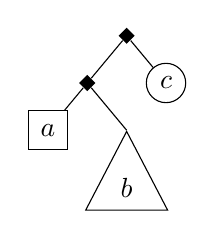
\begin{tikzpicture}[itermtree]
	\node[ap] {} child {
		node[ap] {} child { node[pure] {$a$} } child[subtrm] { node[subtrm] {$b$} }
	} child { node[term] {$c$} };
\end{tikzpicture}
\caption{$(\spure a \sap b) \sap \sterm c$ as a tree.}
\label{fig:iterm-ex}
\end{minipage}\hfill
\begin{minipage}[t]{0.46\textwidth}\centering
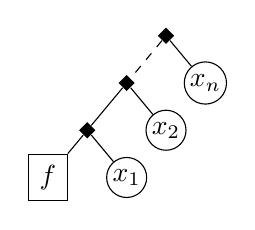
\begin{tikzpicture}[itermtree]
	\node[ap] {} child {
		node[ap] {} child {
			node[ap] {} child {
				node[pure] {$f$}
			} child { node[term] {$x_1$} }
		} child { node[term] {$x_2$} }
	    edge from parent [abbrv]
	} child { node[term] {$x_n$} };
\end{tikzpicture}
\caption{A term in canonical form.}
\label{fig:iterm-nf-ex}
\end{minipage}
\end{figure}

Idiomatic terms are visualized naturally as trees.
This will be helpful in explaining term transformations.
Figure~\ref{fig:iterm-ex} shows the conventions:
Inner nodes correspond to $\sap$, leaves are either pure terms (boxes) or
opaque terms (circles).
Whole subterms may be abbreviated by a triangle.
A term has canonical form if it consists of a single pure node to which a number
of opaque terms (or none) are applied in sequence.
Figure~\ref{fig:iterm-nf-ex} gives a general example.
A formal construction follows:

\begin{definition}[Canonical form]
The set $\mathcal{C} \subset \mathcal{I}$ of idiomatic terms in canonical form
is defined inductively as
\begin{gather}
	\spure x \in \mathcal{C}, \label{eq:cf-base}\\
	t \in \mathcal{C} \implies t \sap \sterm s \in \mathcal{C}. \label{eq:cf-step}
\end{gather}
\end{definition}

\begin{figure}\centering
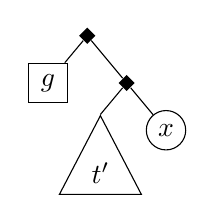
\begin{tikzpicture}[itermtree]
	\node[ap] {} child { node[pure] {$g$} } child {
		node[ap] {} child[subtrmn] { node[subtrm] {$t'$} } child { node[term] {$x$} }
	};
\end{tikzpicture}
\raisebox{10mm}{$\qquad\simeq\qquad$}
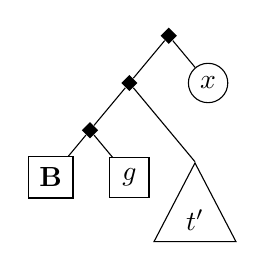
\begin{tikzpicture}[itermtree]
	\node[ap] {} child {
		node[ap] {} child {
			node[ap] {} child { node[pure] {$\mathbf{B}$} } child { node[pure] {$g$} }
		} child[subtrmf] { node[subtrm] {$t'$} }
	} child { node[term] {$x$} };
\end{tikzpicture}
\raisebox{10mm}{$\qquad\simeq\qquad$}
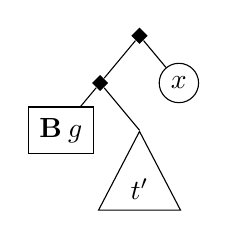
\begin{tikzpicture}[itermtree]
	\node[ap] {} child {
		node[ap] {} child { node[pure] {$\mathbf{B} \sapp g$} } child[subtrm] { node[subtrm] {$t'$} }
	} child { node[term] {$x$} };
\end{tikzpicture}
\caption{The ``pure-rotate'' step.}
\label{fig:pure-rotate}
\end{figure}

It is not entirely obvious how a canonical form can be derived from equations
\eqref{eq:iterm-id}--\eqref{eq:iterm-xchng}.
Rewriting blindly with these is prone to infinite recursion.
Therefore we need a more controlled algorithm.
As we have said before, we use \emph{normal form} to refer to the particular
canonical form derived from those equations.
Consider an idiomatic term $t$.
If $t$ is a single pure term, then it is already in normal form.
The case $t = \sterm x$ is also easy:
Due to \eqref{eq:iterm-id}, we have $t \simeq \spure{(\sabs{x}{x})} \sap t$,
which is in normal form.
But in the case of $t = u \sap v$, various steps could be performed,
depending on the subterms.
We simplify the situation by normalizing each subterm recursively, so we get
an equivalent term $u' \sap v'$ where $u',v' \in \mathcal{C}$.

Now let us assume that $u'$ is just $\spure g$.
If $v'$ is also a pure term, they can be combined along \eqref{eq:iterm-morph}.
Otherwise, the term looks like the one on the left of Figure~\ref{fig:pure-rotate}.
As is shown there, the term tree can be rotated such that one opaque term moves
to the outer-most level.
This is the same equivalence as stated in \eqref{eq:pure-rotate}.
Because the remaining part again has the shape ``pure term applied to normal
form'', we proceed recursively.
In pattern-matching style, the transformation `pure-nf' reads
\begin{align}
	\operatorname{pure-nf}(\spure g \sap (f \sap x)) &=
		\operatorname{pure-nf}{(\spure{(\mathbf{B} g)} \sap f)} \sap x \\
	\operatorname{pure-nf}(\spure f \sap \spure x) &= \spure{(f x)}
\end{align}
\begin{lemma}\label{thm:pure-nf}
For all $g \in \mathcal{T}$ and $t \in \mathcal{C}$,
$\operatorname{pure-nf}(\spure g \sap t)$ is well-defined, and%
\/\footnote{$a \in S \simeq b$ abbreviates ``$a \in S$ and $a \simeq b$''.}
$\operatorname{pure-nf}(\spure g \sap t) \in \mathcal{C} \simeq \spure g \sap t$.
\end{lemma}
\begin{proof}
We prove all claims simultaneously by induction on $t \in \mathcal{C}$,
where $g$ is arbitrary.
\begin{prfcases}
\item Assume $t = \spure x$ for some $x \in \mathcal{T}$.
	Only the second equation applies, so we have
	\[ \operatorname{pure-nf}(\spure g \sap t) = \spure{(g \sapp x)}. \]
	All pure terms are in $\mathcal{C}$, and equivalence follows from
	\eqref{eq:iterm-morph}.
\item Assume $t = t' \sap \sterm x$ for some
	$t' \in \mathcal{C}$, $x \in \mathcal{T}$, and that the hypothesis holds
	for $t'$ and all $g$.
	Only the first equation applies, so
	\[ \operatorname{pure-nf}(\spure g \sap t) =
		\operatorname{pure-nf}(\spure{(\mathbf{B} g)} \sap t') \sap \sterm x. \]
	Instantiating the induction hypothesis, we find that
	\[ \operatorname{pure-nf}(\spure{(\mathbf{B} \sapp g)} \sap t') \in \mathcal{C} \simeq
		\spure{(\mathbf{B} \sapp g)} \sap t' \]
	is well-defined.
	$\mathcal{C}$ is closed under application to opaque terms \eqref{eq:cf-step},
	hence $\operatorname{pure-nf}(\spure g \sap t) \in \mathcal{C}$.
	Finally, we have
	\begin{align*}
		\operatorname{pure-nf}(\spure g \sap t) &\simeq
			\spure{(\mathbf{B} \sapp g)} \sap t' \sap \sterm x \\
		&\stackrel{\mathclap{\eqref{eq:pure-rotate}}}{\simeq}
			\spure g \sap (\spure t' \sap \sterm x) =
			\spure g \sap t. \qedhere
	\end{align*}
\end{prfcases}
\end{proof}

Going back to $u' \sap v'$, we assumed that $u'$ is a pure term.
The case where $v'$ is pure instead can be translated to the former by
\begin{equation}
	\operatorname{nf-pure}(f \sap \spure x) =
		\operatorname{pure-nf}{(\spure{((\sabs{x}\sabs{f}{f x}) \sapp x)} \sap f)} \\
\end{equation}
\begin{lemma}\label{thm:nf-pure}
For all $t \in \mathcal{C}$ and $x \in \mathcal{T}$,
$\operatorname{nf-pure}(t \sap \spure x)$ is well-defined, and
$\operatorname{nf-pure}(t \sap \spure x) \in \mathcal{C} \simeq t \sap \spure x$.
\end{lemma}
\begin{proof}
Follows from Lemma~\ref{thm:pure-nf} and \eqref{eq:iterm-xchng}.
\end{proof}

\begin{figure}\centering
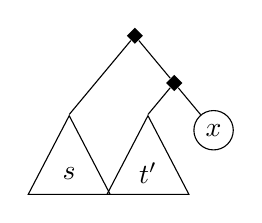
\begin{tikzpicture}[itermtree]
	\node[ap] {} child[subtrmf] { node[subtrm] {$s$} } child {
		node[ap] {} child[subtrmn] { node[subtrm] {$t'$} } child { node[term] {$x$} }
	};
\end{tikzpicture}
\raisebox{10mm}{$\qquad\simeq\qquad$}
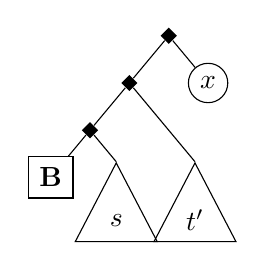
\begin{tikzpicture}[itermtree]
	\node[ap] {} child {
		node[ap] {} child {
			node[ap] {} child { node[pure] {$\mathbf{B}$} } child[subtrmn] {
				node[subtrm] {$s$}
			}
		} child[subtrmf] { node[subtrm] {$t'$} }
	} child { node[term] {$x$} };
\end{tikzpicture}
\caption{The ``rotate'' step.}
\label{fig:rotate}
\end{figure}

Finally, we look at general $u'$, $v'$.
A term rotation is useful again, see Figure~\ref{fig:rotate}.
Before recursion, we must normalize the subterm $\spure \mathbf{B} \sap s$.
But we already know how to do this: by `pure-nf'.
The base case is reached when $v'$ is a single pure term, which is the domain
of `nf-pure'.
The corresponding transformation is therefore
\begin{align}
	\operatorname{nf-nf}(g \sap (f \sap x)) &=
		\operatorname{nf-nf}{(\operatorname{pure-nf}{(\spure \mathbf{B} \sap g)} \sap f)} \sap x \label{eq:nf-nf1}\\
	\operatorname{nf-nf}(t) &= \operatorname{nf-pure}(t) \quad\text{(otherwise)}
\end{align}
\begin{lemma}\label{thm:nf-nf}
For all $s,t \in \mathcal{C}$,
$\operatorname{nf-nf}(s \sap t)$ is well-defined, and
$\operatorname{nf-nf}(s \sap t) \in \mathcal{C} \simeq s \sap t$.
\end{lemma}
\begin{proof}
The proof is similar to the one of Lemma~\ref{thm:pure-nf}, by induction on
$t \in \mathcal{C}$ and arbitrary $s \in \mathcal{C}$.
\begin{prfcases}
\item Assume $t = \spure x$ for some $x \in \mathcal{T}$.
	The second equation applies, so we have
	\[ \operatorname{nf-nf}(s \sap t) = \operatorname{nf-pure}(s \sap \spure x). \]
	Since $s \in \mathcal{C}$, the claim follows directly from Lemma~\ref{thm:nf-pure}.
\item Assume $t = t' \sap \sterm x$ for some
	$t' \in \mathcal{C}$, $x \in \mathcal{T}$, and that the hypothesis holds
	for $t'$ and all $s \in \mathcal{C}$.
	Only the first equation applies,
	\[ \operatorname{nf-nf}(s \sap t) =
		\operatorname{nf-nf} (\operatorname{pure-nf}(\spure \mathbf{B} \sap s) \sap t') \sap \sterm x. \]
	We have
	$\operatorname{pure-nf}(\spure \mathbf{B} \sap s) \in \mathcal{C} \simeq \spure \mathbf{B} \sap s$
	from Lemma~\ref{thm:pure-nf}.
	Thus we can instantiate the induction hypothesis, and the transformed term
	is indeed in normal form.
	Furthermore,
	\begin{align*}
		\operatorname{nf-nf}(s \sap t) &\stackrel{\mathclap{\text{(IH)}}}{\simeq}
			\operatorname{pure-nf}(\spure \mathbf{B} \sap s) \sap t' \sap \sterm x \\
		&\simeq \spure \mathbf{B} \sap s \sap t' \sap \sterm x \\
		&\stackrel{\mathclap{\eqref{eq:iterm-comp}}}{\simeq}
			s \sap (t' \sap \sterm x) = s \sap t. \qedhere
	\end{align*}
\end{prfcases}
\end{proof}

\begin{algorithm}[t]
\caption{Normalization of idiomatic terms.}
\label{alg:normalize}
\begin{gather*}
	\begin{align*}
		\operatorname{normalize}(\spure x) &= \spure x \\
		\operatorname{normalize}(\sterm x) &= \spure{(\sabs{x}{x})} \sap \sterm x \\
		\operatorname{normalize}(x \sap y) &=
			\operatorname{nf-nf}(\operatorname{normalize} x \sap \operatorname{normalize} y)
	\end{align*} \\[2ex]
	\begin{align*}
		\operatorname{nf-nf}(g \sap (f \sap x)) &=
			\operatorname{nf-nf}{(\operatorname{pure-nf}{(\spure \mathbf{B} \sap g)} \sap f)} \sap x \\
		\operatorname{nf-nf}(t) &= \operatorname{nf-pure}(t) \quad\text{(otherwise)}
	\end{align*} \\[2ex]
	\begin{align*}
		\operatorname{pure-nf}(\spure g \sap (f \sap x)) &=
			\operatorname{pure-nf}{(\spure{(\mathbf{B} g)} \sap f)} \sap x \\
		\operatorname{pure-nf}(\spure f \sap \spure x) &= \spure{(f x)}
	\end{align*} \\[2ex]
	\operatorname{nf-pure}(f \sap \spure x) =
		\operatorname{pure-nf}{(\spure{((\sabs{x}\sabs{f}{f x}) \sapp x)} \sap f)}
\end{gather*}
\end{algorithm}

Algorithm~\ref{alg:normalize} summarizes all pieces of the normal form
transformation.
`normalize' is the entry point and performs the main recursion mentioned in the
beginning.
We haven't proved the desired property for `normalize' yet, but this is just a
straightforward induction.

\begin{lemma}\label{thm:normalize}
For all $t \in \mathcal{I}$, $\operatorname{normalize} t$ is well-defined, and
$\operatorname{normalize} t \in \mathcal{C} \simeq t$.
\end{lemma}
\begin{proof}
By induction on $t$, Lemma~\ref{thm:nf-nf}, and equation \eqref{eq:iterm-id}.
\end{proof}

At this point, we know that it is always possible to obtain a certain canonical
form.
This is not sufficient to setup the complete proving process, though.
We need to learn a bit more about the structure of idiomatic terms and how it
relates to lifting.

\begin{definition}[Opaque subterms]\label{def:opaque-seq}
The sequence of opaque subterms of an idiomatic term is defined by the
recursive function
\[
	\operatorname{opaq}(\spure x) = [], \quad
	\operatorname{opaq}(\sterm x) = [x], \quad
	\operatorname{opaq}(s \sap t) = \operatorname{opaq} s @ \operatorname{opaq} t.
\]
$@$ denotes concatenation of lists.
\end{definition}

\begin{definition}[Unlifting]\label{def:unlifting}
Let $t$ be some idiomatic term, and $n = |\operatorname{opaq} t|$.
Let $v_{i \in \{1..n\}}$ be new variable symbols that do not occur anywhere in
$t$.
The ``unlifted'' lambda term corresponding to $t$ is defined as
\[ \unlift{t} = \sabs{v_1} \cdots \sabs{v_n}{\operatorname{vary}_1 t}, \]
where
\begin{align}
	\operatorname{vary}_i (\spure x) &= x, \\
	\operatorname{vary}_i (\sterm x) &= v_i, \\
	\operatorname{vary}_i (s \sap t) &=
		(\operatorname{vary}_i s) \sapp (\operatorname{vary}_{i + |\operatorname{opaq} s|} t).
\end{align}
\end{definition}

\begin{example}\label{exmp:unlift}
The definition of $\downarrow$ may need some explanation.
Consider the idiomatic term
\[ t \equiv \spure{f} \sap x \sap (\spure{g} \sap y \sap z). \]
Its unlifted term is
\[ \unlift{t} = \sabs{a}\sabs{b}\sabs{c}{f \sapp a \sapp (g \sapp b \sapp c)}. \]
The applicative structure is the same, but all opaque terms have been
substituted for new bound variables, which are assigned from left to right.
We do not define lifting formally here, but it should be clear that this is
some sort of inverse operation, given that variables appear only once.
\end{example}

The interesting properties about these two concepts is that they are preserved
by the equivalence relation $\simeq$, and can be directly read from the
canonical form.
Furthermore, we can leverage them to show the uniqueness of the normal form.

\begin{lemma}\label{thm:unlift-equiv}
For equivalent terms $s \simeq t$, the sequences of opaque terms are equivalent
w.r.t $\termeq$, and $\unlift{s} \termeq \unlift{t}$.
\end{lemma}
\begin{proof} (Sketch.)
By induction on the relation $s \simeq t$, where we show
$\operatorname{vary}_i s \termeq \operatorname{vary}_i t$ instead.
The index $i$ is arbitrary.
The part regarding opaque terms is shown easily for each case:
We note that in \eqref{eq:iterm-id}--\eqref{eq:iterm-xchng}, the opaque terms
are identical for both sides.
By the induction hypothesis, this is also true for the necessary closure rules
for symmetry, transitivity, and substitution.
It is obvious that \eqref{eq:termeq-lift} also preserves opaque terms.
Regarding unlifted terms, we have
\begin{prfcases}
\item \eqref{eq:iterm-id}
	\[ \operatorname{vary}_i (\spure{(\sabs{x}{x})} \sap x) =
		(\sabs{x}{x}) \sapp (\operatorname{vary}_i x) \termeq \operatorname{vary}_i x. \]
\item \eqref{eq:iterm-comp}
	Let $j = i + |\operatorname{opaq} g|$ and $k = j + |\operatorname{opaq} f|$.
	\begin{align*}
		\operatorname{vary}_i (\spure \mathbf{B} \sap g \sap f \sap x) &=
		\mathbf{B} \sapp (\operatorname{vary}_i g) \sapp (\operatorname{vary}_j f) \sapp (\operatorname{vary}_k g) \\
		&\termeq (\operatorname{vary}_i g) \sapp ((\operatorname{vary}_j f) \sapp (\operatorname{vary}_k g)) \\
		&= \operatorname{vary}_i (g \sap (f \sap x)).
	\end{align*}
\item \eqref{eq:iterm-morph} and \eqref{eq:iterm-xchng} are similar.
\item \eqref{eq:termeq-lift} By induction.
\item Symmetry, transitivity, and substitution: These follow from the induction
	hypothesis and the corresponding properties of $\termeq$.
\end{prfcases}
\end{proof}

\begin{lemma}\label{thm:unlift-head}
Let $\spure f$ be the single pure term in $t \in \mathcal{C}$.
Then $f \termeq \unlift{t}$.
\end{lemma}
\begin{proof}
By induction on $\mathcal{C}$.
The base case is trivial.
For the step case, we need to prove that
\[ f' \termeq \unlift{(g \sap \sterm x)} =
	\sabs{v_1} \dots \sabs{v_n} \sabs{v_{n+1}}{(\operatorname{vary}_1 g) \sapp v_{n+1}}, \]
where $\spure f'$ is the single pure term in $g$, $n = |\operatorname{opaq} g|$,
and $v_i$ are new variables.
The right-hand side can be eta-reduced to
\[ \sabs{v_1} \dots \sabs{v_n}{(\operatorname{vary}_1 g)} = \unlift{g}. \]
From the induction hypothesis we get $f' \termeq \unlift{g}$, which
concludes the proof.
\end{proof}

This lemma is why we need eta-equivalence and not just use $=_{\alpha\beta}$.
In fact, we can find a counterexample of equivalent canonical forms that do
not agree in the pure function if $\to_\eta$ is not available:
\[ \spure{(\sabs{x}{x})} \sap (\spure f \sap x) \simeq
	\spure f \sap x \simeq \spure{(\sabs{x}{f \sapp x})} \sap x. \]
The middle term is derived from \eqref{eq:iterm-id}, the latter from
\eqref{eq:iterm-comp}.

\begin{corollary}\label{thm:nf-unique}
The normal form is structurally unique.
Formally, if $s,t \in \mathcal{C}$ and $s \simeq t$, then $s \termeq t$.
\end{corollary}

Now we have all tools ready to complete the picture.
The following theorem shows that (limited) lifting is possible with just
the applicative laws.
Its proof hints towards the implementation in Isabelle, which is of course
based on the normal form:
Under the condition that the opaque terms are equivalent, normalizing two
idiomatic terms reduces the problem to the ``unlifted'' terms.

\begin{theorem}\label{thm:nf-lifting}
Let $s,t \in \mathcal{I}$ with $\operatorname{opaq} s \termeq \operatorname{opaq} t$.
If $\unlift{s} \termeq \unlift{t}$ (the base equation), then $s \simeq t$.
\end{theorem}
\begin{proof}
From Lemma~\ref{thm:normalize} we obtain normal forms $s' \simeq s$ and
$t' \simeq t$.
With the base equation and Lemma~\ref{thm:unlift-equiv} we get
$\unlift{s'} \termeq \unlift{t'}$.
By Lemma~\ref{thm:unlift-head} and the condition on the opaque subterms, it
follows that $s' \termeq t'$ and further $s \simeq t$.
\end{proof}

\subsection{Implementation}\label{subsec:nf-implementation}  % TODO title?

We introduced an algorithm for computing the normal form of an idiomatic term,
and argued for its central role in lifting.
In order to be useful in the context of theorem proving, just providing the
normal form is not sufficient.
We need to establish a formal proof of the equivalence.
In Isabelle, this means constructing a theorem $t = t'$, where $t'$ is the
normal form of $t$.
We observe that in Algorithm~\ref{alg:normalize} each equation can be recast
in the following way:
The input term is first transformed in a fixed way that changes the outermost
constitution.
Then, the whole term or subterms thereof are substituted by other functions%
---or recursively---, possibly multiple times.
For instance, in the first equation \eqref{eq:nf-nf1} for nf-nf, the term
$g \sap (f \sap x)$ (where $g$, $f$, $x$ should be understood as placeholders
for concrete terms) is rearranged to $\spure \mathbf{B} \sap g \sap f \sap x$.
The subterm $\spure \mathbf{B} \sap g$ is passed to pure-nf and replaced by
the result, say $g'$.
nf-nf acts on $g' \sap f$, yielding $f'$, such that the final term is
$f' \sap x$.

\begin{table}[t]\centering\small
\begin{tabular}{lrcll}
Function & Pattern & & Substitution & Name \\
\hline
normalize & $\sterm x$ & $\simeq$ & $\spure{(\sabs{x}{x})} \sap \sterm x$ \\
	& $\svar{x}$ & $=$ & $\pure{(\abs{x}{x})} \ap \svar{x}$ & \texttt{I\_intro} \\[1ex]
nf-nf & $g \sap (f \sap x)$ & $\simeq$ & $\spure \mathbf{B} \sap g \sap f \sap x$ \\
	& $\svar{g} \ap (\svar{f} \ap \svar{x})$ & $=$ & $\pure{(\abs{g f x}{g (f x)})} \ap \svar{g} \ap \svar{f} \ap \svar{x}$ & \texttt{B\_intro} \\[1ex]
pure-nf & $\spure g \sap (f \sap x)$ & $\simeq$ & $\spure{(\mathbf{B} \sapp g)} \sap f \sap x$ \\
	& $\pure \svar{g} \ap (\svar{f} \ap \svar{x})$ & $=$ & $\pure{(\abs{f x}{\svar{g} (f x)})} \ap \svar{f} \ap \svar{x}$ & \texttt{B\_pure} \\[1ex]
pure-nf & $\spure f \sap \spure x$ & $\simeq$ & $\spure{(f \sapp x)}$ \\
	& $\pure \svar{f} \ap \pure \svar{x}$ & $=$ & $\pure{(\svar{f} \svar{x})}$ & \texttt{merge} \\[1ex]
nf-pure & $f \sap \spure x$ & $\simeq$ & $\spure{((\sabs{x}{\sabs{f}{f \sapp x}}) \sapp x)} \sap f$ \\
	& $\svar{f} \ap \pure \svar{x}$ & $=$ & $\pure{(\abs{f}{f \svar{x}})} \ap \svar{f}$ & \texttt{swap}
\end{tabular}
\caption{Fixed transformations of Algorithm~\ref{alg:normalize}, with
corresponding rewrite rules. Identity cases are omitted.}
\label{tab:normalize-rules}
\end{table}

Table~\ref{tab:normalize-rules} shows all initial transformations.
It is no coincidence that these are the well-known equivalences
\eqref{eq:iterm-id}--\eqref{eq:iterm-xchng} and~\eqref{eq:pure-rotate}, which
were used in the correctness proofs.
Each transformation has been augmented with the corresponding HOL equation.
The mapping from syntactic idiomatic terms to HOL terms is obvious;
$\pure$ and $(\ap)$ are the concrete constants of the idiom under consideration.
The variables standing for arbitrary opaque terms become new schematic variables,
representing unknowns which may be instantiated.
%$\mathbf{B}$ has been unfolded, ...
Rule \texttt{B\_pure} is easily proven by rewriting with \texttt{B\_intro} and
\texttt{merge}.
The other rules are the applicative laws and thus are available from the
registration infrastructure, see also \todo. % TODO ref to design section
Applying a transformation to a term means instantiating the rule such that the
left hand side is equal to that term.
Isabelle provides a low-level reasoning framework for combining \emph{conversions}~
\cite{paulson83}, which we use here.
A conversion is a function which takes a term $t$ and returns a theorem
$t = u$ for some $u$.%
\footnote{Isabelle's conversions use the Pure equality $\equiv$.}
The ML function \verb+Conv.rewr_conv+ turns a proven equation into such a
conversion function.
When the resulting conversion is applied, it attempts to instantiate the
schematic variables in the equation.
Note that conversions can fail; here if there is no match.
Basic conversion combinators are the \verb+then_conv+ operator, which chains
two conversions sequentially (and fails if any of these does),
and the \verb+else_conv+ operator, which attempts to apply the first conversion,
but uses the second if the first fails.
%\verb+Conv.all_conv+ is the identity of \verb+then_conv+; ...
Because rewrite conversions act like pattern matching guards, we combine them
with \verb+else_conv+ to recreate the case switching of the algorithm.
Combinators like \verb+Conv.arg1_conv+ facilitate the rewriting of subterms---%
this one takes a conversions and modifies it such that it applies to the left
operand of a binary operator.
With these tools at hand, we can construct the normal form conversion.
The recursive pieces can be expressed just as recursive auxiliary functions.
However, we lose a bit of generality by using \verb+Conv.arg1_conv+ to access
the left operand of $(\ap)$, because it requires that $(\ap)$ is not a
beta-redex.
This could be solved by creating a specialized combinator, which does pattern
matching instead of simple term deconstruction.

\begin{figure}
\begin{lstlisting}[language=ml]
fun normalform_conv ctxt af =
  let
    val rules = facts_of_afun af;

    val leaf_conv = rename_rewr_conv (fn t => [("x", term_to_vname t)])
      (#I_intro rules);
    val merge_conv = Conv.rewr_conv (#merge rules);
    val swap_conv = Conv.rewr_conv (#swap rules);
    val rotate_conv = rename_rr_conv "x" (#B_intro rules);
    val pure_rotate_conv = rename_rr_conv "x" (#B_pure rules);

    fun normalize_pure_nf ct = ((pure_rotate_conv then_conv
      Conv.arg1_conv normalize_pure_nf) else_conv merge_conv) ct;
    val normalize_nf_pure = swap_conv then_conv normalize_pure_nf;
    fun normalize_nf_nf ct = ((rotate_conv then_conv
        Conv.arg1_conv (Conv.arg1_conv normalize_pure_nf then_conv
          normalize_nf_nf)) else_conv
      normalize_nf_pure) ct;

    fun normalize ct =
      let val t = Thm.term_of ct
      in if can (dest_comb ctxt af) t
        then (Conv.arg1_conv normalize then_conv
            Conv.arg_conv normalize then_conv normalize_nf_nf) ct
        else if can (dest_pure ctxt af) t
          then Conv.all_conv ct
          else leaf_conv ct
      end;
  in normalize end;
\end{lstlisting}
\caption{ML implementation of normalization.}
\label{fig:ml-normalform}
\end{figure}

Figure~\ref{fig:ml-normalform} shows the ML code.
It is parameterized by the applicative functor \verb+af+, which contains all
the necessary rules.
In the helper function \verb+normalize+, the different cases are selected
by predicates like \verb+can (dest_comb ctxt af) t+, which is true only if
term \verb+t+ fits the pattern $\_ \ap_\mathtt{af} \_$.
We do this here because it is the only recursive conversion which is not
guarded by a rewrite rule before recurring, so we want to protect against
rampant rewriting.
Finally, \verb+rename_rewr_conv+ and \verb+rename_rr_conv+ (not shown)
adjust the names of bound variables in the argument rule to the term to convert.
While these names are only hints in Isabelle and obviously subject to alpha
conversion, they influence the display of the proof state.
To elaborate, consider a HOL term $p \ap (q \ap r)$.
Without the adjustment, the normal form would be
$\pure{(\abs{xx_ax_b}{x(x_ax_b)})} \ap p \ap q \ap r$.
The name component $x$ stems from the lambda abstraction in rule \verb+B_intro+.
If the term is part of an equation, the variables of the reduced base equation
will also be called $x$, $x_a$, and $x_b$.
This creates unnecessary confusion, and to help the user, we try to preserve the
variable names of the input term.

\section{Lifting with Combinators}\label{sec:combinators}

\subsection{Motivation}\label{subsec:combinator-motivation}

The normalization approach to solving lifted equations works only if the
opaque terms on both sides coincide.
This is not true for all equations of interest.
Let's revisit the set version of addition of natural numbers, $\oplus$ from
Example~\ref{exmp:set-intro}.
This operator is also commutative, so it should be possible to prove
\[ X \oplus Y = Y \oplus X. \]
After unfolding and normalization, we get
\begin{equation}\label{eq:comb-intro1}
	\pure{(\abs{xy}{x + y})} \ap X \ap Y = \pure{(\abs{yx}{y + x})} \ap Y \ap X.
\end{equation}
Clearly, this can't be solved with a standard congruence rule, because we would
have to to prove that $X$ is equal to $Y$.
Since we are concerned with transferring properties from a base domain,
we don't want to assume anything about those opaque subterms.

Hinze showed that such equations can be solved if certain \emph{combinators}
can be lifted.
Informally, combinators are functions which rearrange their arguments in a
specific manner.
We have already used two combinators, $\mathbf{I}$ and $\mathbf{B}$.
Lifting their defining equations (see Table~\ref{tab:combinators}) gives us
the identity and composition laws, respectively.
If the lifted combinator performs the same rearrangement with arbitrary
functorial values, one can translate that particular term structure between the
two layers.
In this case, we simply say that the combinator \emph{exists}.
To continue with~\eqref{eq:comb-intro1}, we could attempt to change the order of
$Y$ and $X$ on the right-hand side.
Note that these appear as arguments to a pure function.
The $\mathbf{C}$ combinator, also known as `flip' in functional programming,
does what we want: $\mathbf{C}fxy = fyx$.
The lifted equation is
\begin{equation}\label{eq:flip-lifted}
	\pure \mathbf{C} \ap f \ap x \ap y = f \ap y \ap x,
\end{equation}
and it is indeed true for set idiom!
From this we get
\begin{equation}\label{eq:comb-intro2}
	\pure{(+)} \ap X \ap Y = \pure{(\mathbf{C}(+))} \ap X \ap Y.
\end{equation}
The right-hand side is no longer the normal form of $Y \oplus X$, but still
a canonical form (which is why we distinguish these two).
But now the argument lists on both sides coincide.
We reduce to
\[ \abs{xy}{x + y} = \abs{xy}{y + x}, \]
which is extensionally equivalent to the base equation $x + y = y + x$.
The availability of equation~\eqref{eq:flip-lifted} is a quite powerful
condition, because it will allow us to permute opaque terms freely.
If permutations exist such that both sides of an equation in canonical form
align regarding their opaque terms, reduction by congruence is possible again.
This will again lead to the expected base equation.
However, the combinator $\mathbf{C}$ does not exist for all applicative functors.
For example, the order of values in a state monad may be significant.

\begin{table}\centering
\begin{tabular}{cll}
Symbol & Reduction \\
\hline
$\mathbf{B}$ & $\mathbf{B} x y z = x (y z)$ \\
$\mathbf{I}$ & $\mathbf{I} x = x$ \\
\hline
$\mathbf{C}$ & $\mathbf{C} x y z = x z y$ \\
$\mathbf{K}$ & $\mathbf{K} x y = x$ \\
$\mathbf{W}$ & $\mathbf{W} x y = x y y$ \\
$\mathbf{S}$ & $\mathbf{S} x y z = x z (y z)$ \\
$\mathbf{H}$ & $\mathbf{H} x y z = x y (z y)$ \\
\end{tabular}
\caption{Useful combinators.}
\label{tab:combinators}
\end{table}

Combinators appeared originally in the context of logic~\cite{curry68}.
They were studied because it is possible to write logical formulas without
variables using only applications of suitable combinators, as opposed to the
usual lambda calculus.
Table~\ref{tab:combinators} lists all combinators which are used throughout
this text, together with their defining equations.
There are certain sets of combinators which are sufficient to express all
lambda terms, $\{\mathbf{S,K}\}$ being one of them.
In other sets, only a limited part of terms is representable.
Hinze's Lifting Lemma shows that all terms and thus all equations can be
lifted while preserving the variable structure if $\mathbf{S}$ and $\mathbf{K}$
exist.
He also notes that other combinator set are useful, because there are idioms
where more than $\{\mathbf{B,I}\}$, but not all combinators exist.
Generally speaking, additional combinators enlarge the set of equations which
can be lifted.

The original proof of the Lifting~Lemma~\cite[11--14]{hinze10} uses induction
on the structure of idiomatic terms; it is not entirely obvious how it can
be generalized to other combinators sets, as it depends on the availability
of $\mathbf{K}$ to lift tuple projections.
In this section we present an implementation of this generalized lifting,
whose underlying concept works with arbitrary combinators.
However, tt depends on an abstraction algorithm and the structure of
representable terms, which are difficult to derive automatically.
Therefore we will restrict ourselves to certain sets (``bases'') with
fixed algorithms, while understanding that the scope can be extended 
if needed.

\subsection{General Lifting}\label{subsec:general-lifting}

We start with the relationship of combinators and lambda terms.
The equations in Table~\ref{tab:combinators} can be expressed as abstractions
$\mathbf{I} = \abs{x}{x}$ etc.
If we substitute occurrences of combinators in a term, new abstractions are
introduced, which may be beta-reduced afterwards:
\[ \mathbf{WB} = (\abs{fx}{fxx})(\abs{gfx}{g(fx)}) =_\beta \abs{xy}{x(xy)}. \]
The question arises when and how this process can be reversed, meaning that
all abstractions are replaced by suitable combinators.
In Curry et.~al.~\cite[Section~6A]{curry68}, terms with variables, but no
abstractions are considered.
A syntactical operation is defined, denoted $[x]t$, where $t$ is such a term
and $x$ is a variable.
The desired property is that $x$ does not occur in $[x]t$, and
$([x]t)x = t$.  % TODO check Curry - what is = here?
Due to its notation, the operation is known as \emph{bracket abstraction}.
There is an obvious correspondence with lambda abstractions $\abs{x}{t}$.
Bracket abstraction however is defined to evaluate to a concrete applicative
term, whereas a lambda is an object of the syntax itself. % TODO check Curry chapter 3
Replacing lambdas $\abs{x}{t}$ by brackets $[x]t$ performs the shift to a
combinator representation.
Curry et.\ al. give several possible definitions for bracket abstraction.
They note that these follow a scheme they refer to as an algorithm---a sequence
of rules, where each rule is a partial definition.
The rules may invoke abstraction recursively.
In particular, the following rules are used:

\begin{alignat}{2}
	\tag{$i$} [x]x &= \mathbf{I}, && \\
	\tag{$k$} [x]t &= \mathbf{K} t &&\qquad\text{if $x$ not free in $t$}, \\
	\tag{$\eta$} [x]tx &= t &&\qquad\text{if $x$ not free in $t$}, \\
	\tag{$b$} [x]st &= \mathbf{B}s([x]t) &&\qquad\text{if $x$ not free in $s$}, \\
	\tag{$c$} [x]st &= \mathbf{C}([x]s)t &&\qquad\text{if $x$ not free in $t$}, \\
	\tag{$s$} [x]st &= \mathbf{S}([x]s)([x]t). &&
\end{alignat}

The algorithm which consists of rules $(i)$, $(k)$ and $(s)$, in that order,
is written succinctly as $(iks)$.
The algorithm attempts to use the rules in their left-to-right order, applying
the first one whose restrictions are satisfied by the term at hand.
Each abstraction algorithm $A$ introduces a certain set of primitive combinators,
which we refer to as $C(A)$.
It is sound only if certain postulates about those combinators, which are again
the equations in Table~\ref{tab:combinators}, are assumed.

\begin{example}\label{exmp:bracket-abs}
Using the $(iks)$ algorithm, one gets
\[ [x]xxy \stackrel{(s)}{=} \mathbf{S}([x]xx)([x]y)
	\stackrel{(s),(k)}{=} \mathbf{S}(\mathbf{S}([x]x)([x]x))(\mathbf{K}y)
	\stackrel{(i)}{=} \mathbf{S}(\mathbf{SII})(\mathbf{K}y). \]
Attempting to use the $(ik\eta bc)$ algorithm with the same abstraction
quickly comes to a halt:
\[ [x]xxy \stackrel{(c)}{=} \mathbf{C}([x]xx)y, \]
which is undefined.
\end{example}

As we can see, not all algorithms are total.
Therefore, there is a trade-off between the combinators required and the terms
for which abstraction is possible.
Bunder~\cite{bunder96} presents an analysis of the situation for certain
algorithms and combinator sets, based on rigorous definitions for term
translation and definability.
We will come back to this later, when we discuss how to order the variables in
an idiomatic term such that abstraction is defined.
For now, the concept of bracket abstraction with the example of rules
$(i)$--$(s)$ is sufficient.

Next, we attempt to transfer these concepts to idiomatic terms.
On the one hand, this is quite intuitive since the latter are also formed by
an application operator, and pure terms can be identified with constants.
But we do not have any ``idiomatic abstractions''.
Hinze actually defines these in terms of abstract combinators and an
extensionality property of the idiom.
For our purpose it is sufficient to work directly with bracket abstraction,
and we assume that all combinators are lifted, i.e. expressible as a pure term.
To clarify the following discussion, we adjust our $\mathcal{I}$ formalism
and replace opaque terms $\sterm x$ with variables.

\begin{definition}
The set of generic idiomatic terms $\mathcal{I}'$ is defined by
\begin{equation}
	\mathcal{I}' ::= \sivar \mathcal{V} \mid \spure \mathcal{T} \mid
		\mathcal{I}' \sap \mathcal{I}'.
\end{equation}
We reuse the congruence $\simeq$ from Definition~\ref{def:idiomatic-terms} for
generic terms.
The set of variables $\operatorname{var}(t)$ of $t$ is defined as the set of
all arguments to $\sivar$ occuring in $t$.
Unlifting (see Definition~\ref{def:unlifting}) is also transferred, but uses
the variable $x$ in subterms $\sivar x$ instead of inventing new ones.
\end{definition}

Using this definition, it is clear what the rules for idiomatic abstraction
are:
\begin{alignat}{2}
	\tag{$i'$} [x](\sivar x) &= \spure \mathbf{I}, && \\
	\tag{$k'$} [x]t &= \spure \mathbf{K} \sap t &&\qquad\text{if } x \not\in \operatorname{var}(t), \\
	\tag{$b'$} [x](s \sap t) &= \spure \mathbf{B} \sap s \sap [x]t &&\qquad\text{if } x \not\in \operatorname{var}(s), \\
	\tag{$c'$} [x](s \sap t) &= \spure \mathbf{C} \sap [x]s \sap t &&\qquad\text{if } x \not\in \operatorname{var}(t), \\
	\tag{$s'$} [x](s \sap t) &= \spure \mathbf{S} \sap [x]s \sap [x]t. &&
\end{alignat}
In general, the algorithm $A'$ on idiomatic terms is obtained from algorithm
$A$ on regular terms by lifting its rules in this fashion, preserving order.
% TODO lifted combinator defs?
% TODO W combinator 

Before we show the connection to the canonical form, there is one thing which
remains to be considered.
The interchange law allows us to move a variable out of the left subterm of
an application, given that the right subterm is pure.
This is not captured by rules $(b')$ and $(i')$, which are the only ones from
above which are valid in all idioms.
We define a combinator $\mathbf{T}xy = yx$ and the rules
\begin{alignat}{2}
	\tag{$t$} [x]st &= \mathbf{T}t([x]s) &&\qquad\text{if $t$ contains no variables}, \\
	\tag{$t'$} [x](s \sap t) &= \spure \mathbf{T} \sap t \sap [x]s &&\qquad\text{if } \operatorname{var}(t) = \emptyset.
\end{alignat}
Soundness of rule $(t')$ can be shown to be equivalent to the interchange law.
It is important to understand that $\mathbf{T}$ does not have to exist in the
idiom; these rules do not fit exactly in the pattern of the other rules.

As with ordinary terms, we demand a soundness property for idiomatic bracket
abstraction, namely that $[x]t \sap \sivar x \simeq t$ holds.
The required combinator definitions get lifted to $\mathbf{I} \sap x \simeq x$
and so on.
\begin{lemma}
Let $t \in \mathcal{I'}$ be a generic idiomatic term, and $x \in \mathcal{V}$
a variable.
For an abstraction algorithm $A$ consisting of a subset of rules $(i')$--$(t')$,
we have $[x]t \sap \sivar x \simeq t$, assuming that all combinators $C(A)$
exist.
\end{lemma}
\begin{proof}
\todo ?
\end{proof}

Now we can state the key obversation:
The successful abstraction of all variables in an idiomatic term leaves a
single pure term, per the homomorphism law.
Moreover, that term is identical to the result of applying the same abstraction
algorithm to the ``unlifted term''.

\begin{theorem}
In the following, bracket abstraction uses algorithms $A$ and $A'$, respectively.
Let $t \in \mathcal{I}'$ be a generic idiomatic term, and $x_1,\dots,x_n$
a sequence of variables such that $\{x_1,\dots,x_n\} \supseteq \operatorname{var}(t)$.
If $[x_1]\cdots[x_n]t$ is defined for $A'$, then
\begin{enumerate}
\item $[x_1]\cdots[x_n]t$ consists only of applications of pure terms; and
\item the unique canonical form of $[x_1]\cdots[x_n]t$ is $\spure t'$, where
\item $t' = [x_1]\cdots[x_n]\unlift{t}$, thus
\item replacing all combinators from $C(A)$ in $t'$ with their definitions
	yields $t'' \termeq \abs{x_1\cdots x_n}{\unlift{t}}$.
\end{enumerate}
\end{theorem}

\subsection{Combinator Bases}\label{subsec:combinator-bases}

\begin{table}\centering
\begin{tabular}{ll}
Base & Example idioms \\
\hline
$\mathbf{BI}$ & state, list \\
$\mathbf{BIC}$ & set \\
$\mathbf{BIK}$ & \\
$\mathbf{BIW}$ & either \\
$\mathbf{BCK}$ & \\
$\mathbf{BKW}$ & \\
$\mathbf{BICW}$ & maybe \\
$\mathbf{BCKW}$ & stream, $\alpha \to$ \\
\end{tabular}
\caption{Substructures of BCKW.}
\label{tab:combinator-bases}
\end{table}

\todo

\printbibliography

\end{document}
